\chapter{Something else}
\chapter{What is Logic and What is Proof}
We will be learning many seemingly foreign words as we move through the text. It comes up often that we need to name things, and the names themselves should be as specific as possible in meaning.

For this, we will introduce logic as any system with \textbf{epistemic closure}, which more generally speaking, will be any \textbf{preorder}. Now, these words have not yet been defined, and we will ensure that we get there both intuitively and formally. However, it will also be your first opportunity to understand isomorphisms between words and meanings. Effectively, a preorder and an epistemic closure are the same thing, but they are stated in two completely different ways that we will demonstrate are equivalent.

\section{Reachability}

Before we begin describing each, let's talk about the intuitive term \textbf{reachability}; however, in this case, we are talking about reachability that is possibly one way. Imagine yourself on ski slopes. If two paths connect, then you can reach the one that is at your height (by walking) or below (by skiing). However, in our metaphor for reachability, you (and I) are just too lazy to walk uphill, carrying your skis, without your snowshoes.

This metaphor actually describes an anecdote in my life that I was one a ski hill, and fell at the top. My snow boot was inside my ski at the top of the hill, my other ski fell to the bottom of the hill, and I didn't stop myself from falling until I was midway. My first thought was climb to the top, since the climb will be doubly as difficult coming from the bottom.

The slope was freshly groomed, and still icy from the groomer. I fought and pulled myself up for 30 minutes and had only gotten part of the way up, until some other skier came to the top of the slope, saw the ski and shoe, and decided to help by bringing it to me.

Afterwards, continuing my descent (my tumble) down the hill was fairly easy, and I reached my other ski, put myself back together, and started skiing again.

When we are discussing reachability, we are often describing things that are both one-way, and things that are two-way. However, it cannot be readily assumed that reaching one thing means that I can reach back.

Now, you may be wondering why, if these two ideas are isomorphic, and hence definitively equivalent, why do we have 2 words for the same concept. There is some historical history that's even more apparent when we consider that a logic system \emph{has} epistemic closure and \emph{is} a preorder. However, this historic reasons are not the only reason.

The word closure, when attached to epistemic, will make more sense when we define what closure means in the subject of Topology, and the word preorder will make more sense when discuss the subject of Order Theory. They are two different mental approaches that got reunited again later, and we are looking back with 20/20 vision, reuniting them at the beginning of this book.

\begin{definition}
An epistemic closure means that if we start with something `a' and we know that we can reach `b' from `a', then we can get to `b'.
\end{definition}

\begin{align*}
    a \leadsto b & \quad & \text{means that `a' leads to `b'} \\
    a & \quad & \text{means that we can reach `a'}\\
    \vdash b & \quad & \text{therefore we can reach `b'}
\end{align*}

Some examples of epistemic closure include:
\begin{itemize}
    \item From a starting point of a path, and a path connecting the starting point to the destination, we can get to the destination
    
    \item Given some starting information, and that this information always implies some conclusion, we can reach the conclusion
    
    \item Given that a first value is large enough, and a second value is larger, then the second value is large enough.
    
    \item A diagram drawn to represent reachability allows us to start at a location, and reach another location from it.
\end{itemize}

The definition of a preorder requires a few additional things, and requires that we actually talk about about ``reflextivity'' and ``transitivity'' first.

\begin{definition}
The concept of being reachable has the property of being \textbf{reflexive} such that if our starting point and destination are the same ($a \leadsto a$), then we can reach our destination.
\end{definition}

More formally:
\begin{align*}
    a \leadsto a & \quad & \text{means that `a' leads to `a'} \\
    a & \quad & \text{means that we can reach `a'}\\
    \vdash a & \quad & \text{therefore we can reach `a'}
\end{align*}

\begin{definition}
The concept of being reachable has the property of being \textbf{transitive}, such that if we can get to `b' from `a' and we can get to `c' from `b', then we can get to `c' from `a' (i.e. $(a\leadsto b, b \leadsto c)\vdash a \leadsto c$
\end{definition}

More formally:
\begin{align*}
    a \leadsto b \\
    a \\
    \vdash b \\
    \\
    b \leadsto c \\
    b \\
    \vdash c
\end{align*}

Now, I can see some friends of mine saying, ``That's just common sense'', and at this point, I'd agree. However, mathematics and philosophy are often in the business of formally stating ``common sense'' and then proving it or disproving it.

\section{Mathematical Categories}

Since we are discussing logic and preorders, there is no reason why we shouldn't also introduce a category. Earlier, in the examples of epistemic closure, I mentioned diagrams that represented reachability. Such a diagram may look like this:



\tikzset{every picture/.style={line width=0.75pt}} %set default line width to 0.75pt        

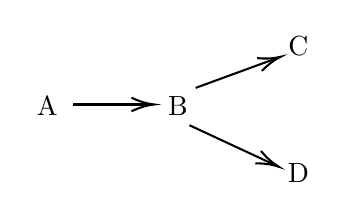
\begin{tikzpicture}[x=0.75pt,y=0.75pt,yscale=-1,xscale=1]
%uncomment if require: \path (0,300); %set diagram left start at 0, and has height of 300

%Straight Lines [id:da8530145644356999] 
\draw    (132.5,149) -- (169.5,149) ;
\draw [shift={(171.5,149)}, rotate = 180] [color={rgb, 255:red, 0; green, 0; blue, 0 }  ][line width=0.75]    (10.93,-3.29) .. controls (6.95,-1.4) and (3.31,-0.3) .. (0,0) .. controls (3.31,0.3) and (6.95,1.4) .. (10.93,3.29)   ;

%Straight Lines [id:da2900632045462661] 
\draw    (191.5,141) -- (230.62,126.69) ;
\draw [shift={(232.5,126)}, rotate = 519.9] [color={rgb, 255:red, 0; green, 0; blue, 0 }  ][line width=0.75]    (10.93,-3.29) .. controls (6.95,-1.4) and (3.31,-0.3) .. (0,0) .. controls (3.31,0.3) and (6.95,1.4) .. (10.93,3.29)   ;

%Straight Lines [id:da9565637858295115] 
\draw    (188.5,159) -- (229.69,178.16) ;
\draw [shift={(231.5,179)}, rotate = 204.94] [color={rgb, 255:red, 0; green, 0; blue, 0 }  ][line width=0.75]    (10.93,-3.29) .. controls (6.95,-1.4) and (3.31,-0.3) .. (0,0) .. controls (3.31,0.3) and (6.95,1.4) .. (10.93,3.29)   ;

\draw (120,150) node  [align=left] {A};
\draw (183,150) node  [align=left] {B};
\draw (241,121) node  [align=left] {C};
\draw (241,182) node  [align=left] {D};

\end{tikzpicture}

Here, we see a directed graph that leads us from A to B, and a choice to go from B to C or from B to D. We know that we can reach A from A, B from B, C from C, and D from D. We also know that we can reach B, C, and D from A. Finally, we know that we can reach C and D from B.

\begin{definition}
    A \textbf{directed graph} is a diagram with objects and arrows where the arrows indicate direction. An \textbf{undirected graph} would not require arrows, or would be arrows that go in both directions.
\end{definition}

\begin{definition}
    In mathematics, a \textbf{category} is a directed graph that requires that each object can reach itself (reflexivity), and that if we can reach one object that reaches another, that we can reach that second object (transitivity).
\end{definition}

Therefore, a category is a diagram that uses the same properties as a preorder, which we have also established, are the same properties as epistemic closure.

This allows us to take logic and draw diagrams that represent what the logical statements say. It also means that we can diagrammatically describe a preorder as well.

